\section{Introduktion}
Netværklaget omhandler en host-to-host kommunikation service dvs. dens opgave består i at sende pakker fra en ‘sending host’ til en ‘receiving host’.
\begin{center}
  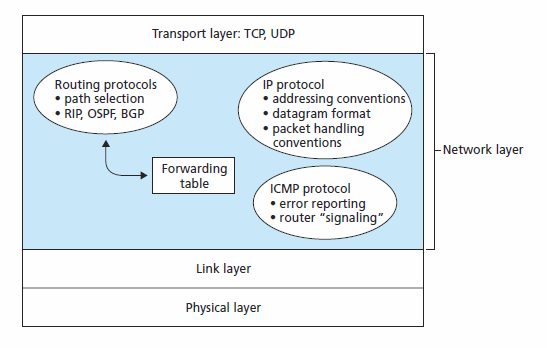
\includegraphics{4-network-layer/networklayer.png}
\end{center}
\begin{itemize}
	\item host-to-host kommmunikation
	\item forbindelsesorienteret (eks. telefonsamtale) - pålidelig
	\item forbindelsesløs - upålidelig
	\item videresendelse
	\item stibestemmelse
	\item connection setup
\end{itemize}

\section{Netværk service modeller}
\begin{itemize}
	\item guaranteed delivery
	\item guaranteed delivery with bounded delay
	\item Internettet
	\item Constant bitrate (CBR)
	\item Available Bit Rate (ABR)
\end{itemize}

\section{Pakkekoblede netværk}
\begin{itemize}
	\item datagramnetværk 
	\item virtuelle kredsløbs koblede netværk
	\item Internettet
	\item Constant bitrate (CBR)
	\item Available Bit Rate (ABR)
\end{itemize}

\subsection{Virtuelle kredsløbs koblede netværk}
{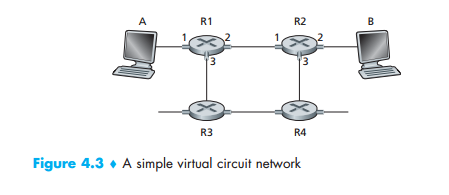
\includegraphics{4-network-layer/vc-network.png}
\begin{itemize}
	\item rute 
	\item VC nummer
	\item videresendelsestabel
	\item 3 faser - VC setup - Data transfer - VC teardown
	\item opbevarer oplysninger om forbindelsesstatus
	\item videresendes ud fra den forbindelsen pakken tilhører
\end{itemize}
{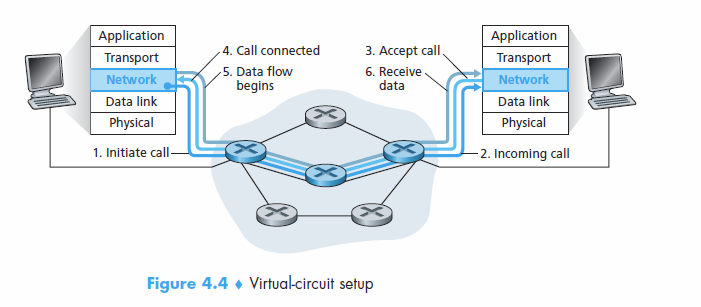
\includegraphics{4-network-layer/vc-network-3faser.png}

\subsection{Datagramnetværk}
{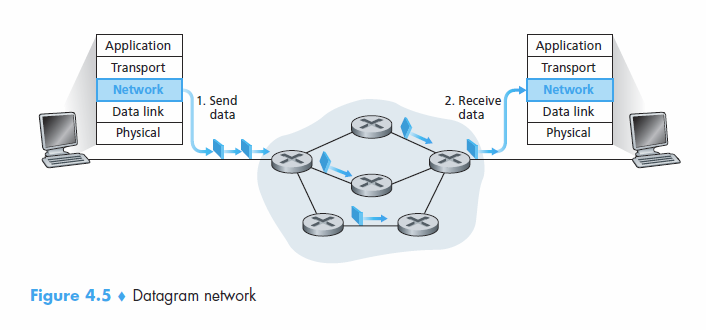
\includegraphics{4-network-layer/datagramnetwork.png}
\begin{itemize}
	\item kun kendt for de to slutsystemer
	\item header (hierarkisk sturktur) 
	\item videresendelsestabel
	\item eks. med postvæsenet
	\item ikke garanti for rigtig rækkefølge
	\item opbevarer INGEN oplysninger om forbindelsesstatus
	\item videresendes ud fra modtageradressen
\end{itemize}

\section{Routingprincipper}
Bestemmelsen af routen er en opgave der tilhører routingprotokollen, eller nærmere bestemt den routingalgoritme der er en del af routingprotokollen.
\begin{itemize}
	\item transportere datagrammer
	\item bestemmelse af route (routingprotokollen)
	\item Global routingalgoritme – Link state algoritmer
	\item Decentral routingalgoritme – Distance vektor algoritmer
\end{itemize}

\subsection{Global routingalgoritme – Link state algoritmer}
\begin{itemize}
	\item Den billigste sti mellem afsender og modtager
	\item global
	\item broadcast
	\item routing tabel
	\item dynamisk
\end{itemize}

\subsection{Decentral routingalgoritme – Distance vektor algoritmer}
\begin{itemize}
	\item Den hurtigste sti fra afsender til modtager
	\item iterativ og distribueret
	\item ingen kendskab til omkostningerne i netværket
	\item naboer
	\item kender ikke den komplette sti
	\item statisk
	\item asynkron
	\item distancetabel
\end{itemize}
\begin{center}
  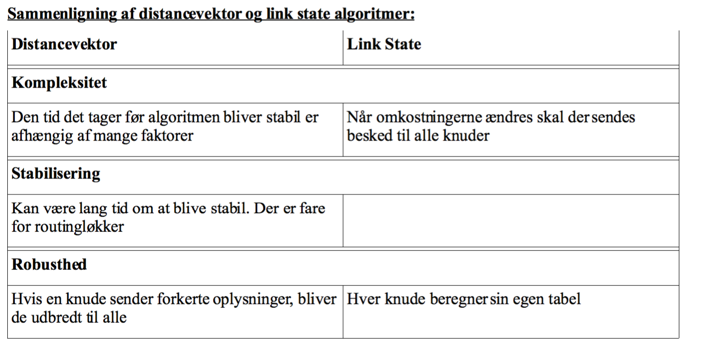
\includegraphics[scale=0.8]{4-network-layer/sammenligning-link-state-distance-vektor.png}
\end{center}


\section{Sådan virker en router}
En router er en enhed på et computernetværk som forbinder et antal logiske eller fysiske netværk ved at videresende pakker fra et netværk til deres destination på et andet netværk i en process kaldet routing. Routeren arbejder på OSI-modellens lag 3 (netværkslaget), i internetprotokollen kaldes dette lag IP-laget.
\begin{center}
  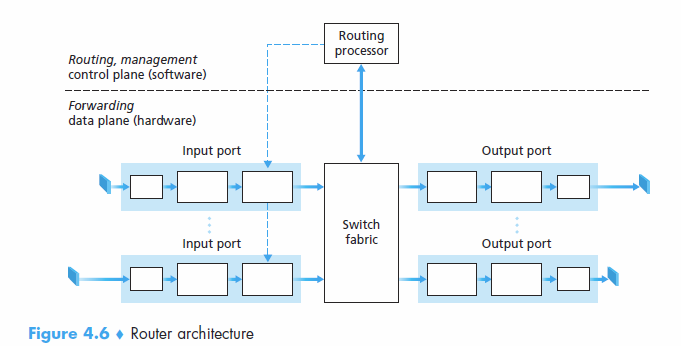
\includegraphics[scale=0.8]{4-network-layer/whats-inside-a-router.png}
\end{center}
\begin{itemize}
	\item input ports
	\item switching fabric
	\item output ports
	\item routing processor
	\item packet scheduler(opfyldelsesgaranti, isolere 'flows' fra hinanden)
	\item packet scheduler algoritmer(FCFS - WFQ - RR)
	\item QoS
\end{itemize}
{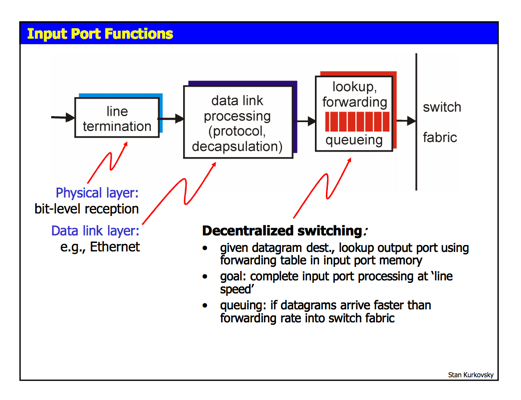
\includegraphics{4-network-layer/router-input-port}
{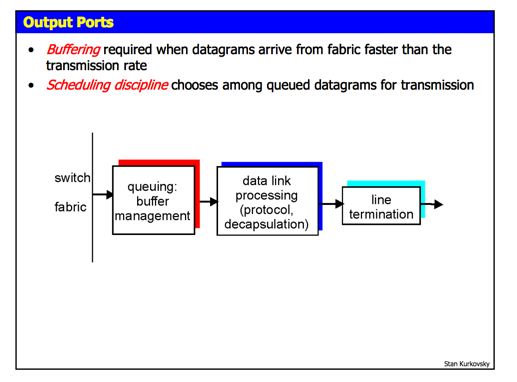
\includegraphics{4-network-layer/router-output-port.png}

\section{Hierarkisk routning}
En router er en enhed på et computernetværk som forbinder et antal logiske eller fysiske netværk ved at videresende pakker fra et netværk til deres destination på et andet netværk i en process kaldet routing. Routeren arbejder på OSI-modellens lag 3 (netværkslaget), i internetprotokollen kaldes dette lag IP-laget.
\begin{center}
  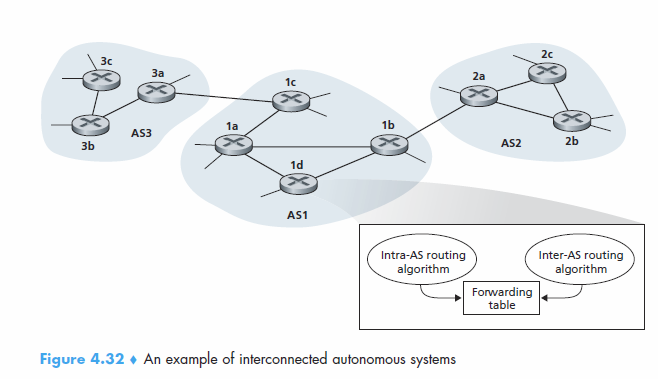
\includegraphics[scale=0.8]{4-network-layer/hierarkisk-routing.png}
\end{center}
\begin{itemize}
	\item autonome systemer(AS)
	\item klassificeret i regioner(reducere hukommelses krav)
	\item intraautonom system routing protokol
	\item hot-potato routing(hurtigt og lave omkostninger - pakke => gatewayrouter)
\end{itemize}

\section{Internetprotokollen – IP}
Den protokol der bruges på internettets netværkslag er IP protokollen. 
Derfor kaldes internettets netværkslag også for IP-laget. Internetprotokollen er imidlertid bare en del af internettets netværkslag, der består af 3 hovedkomponenter.
\begin{center}
  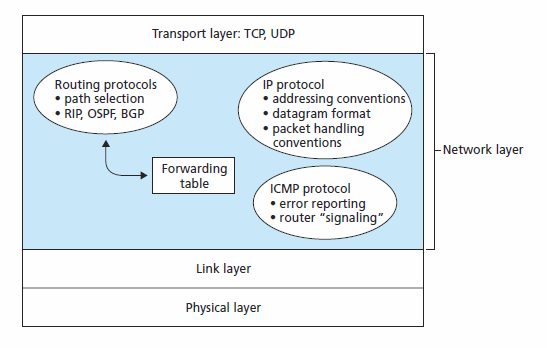
\includegraphics{4-network-layer/networklayer.png}
\end{center}
\begin{itemize}
	\item Internet Protocol(adressering - felter i datagrammet - IPv4 - IPv6)
	\item Stibestemmelse(beregne pakke sti - vedligeholdelse af netværket)
	\item Fejlrapportering(rapportere  fejl i datagrammet - ICMP
\end{itemize}

\section{IPv4 adressering}
En vært er sædvanligvis koblet til netværket med én forbindelse. Grænsen mellem værten og det fysiske netværk kaldes en interface.
\begin{center}
  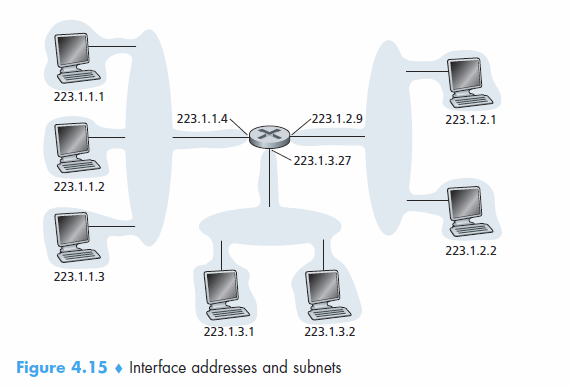
\includegraphics{4-network-layer/ipv4-adressering.png}
\end{center}
\begin{itemize}
	\item Interface
	\item IP adressen knyttet til interfacet
	\item IP addresse 32 bits, dotted decimal format
	\item Netværksprefikset
	\item Værtsdel
	\item Netværksmasken
	\item 5 netklasser(specifikt adresseområde - variable felter)
	\item Subnet mask(host og net delen)
\end{itemize}
{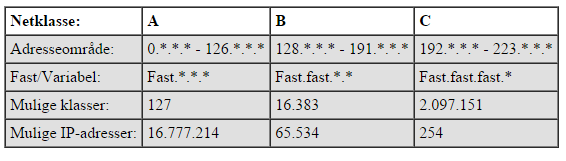
\includegraphics{4-network-layer/netklasser.png}
\begin{center}
  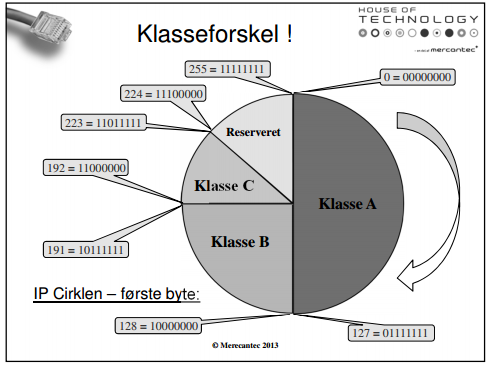
\includegraphics{4-network-layer/klasseforskel.png}
\end{center}
{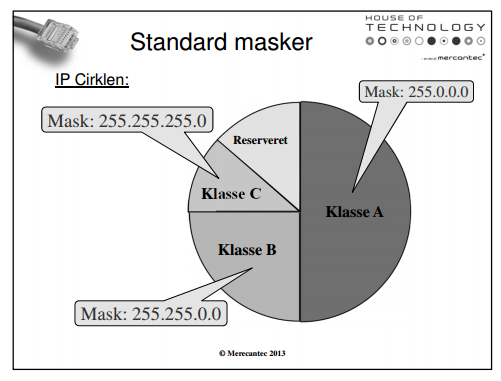
\includegraphics{4-network-layer/masker.png}

\section{Tildeling af IP adresser}
\begin{itemize}
	\item Manuel konfiguration
	\item Dynamic Host Configuration Protocol – DHCP(plug-and-play protokol - flere brugere - færre ip adresser - let at administrerer - adressekonflikt)
\end{itemize}

\section{Ipv4 datagram}
{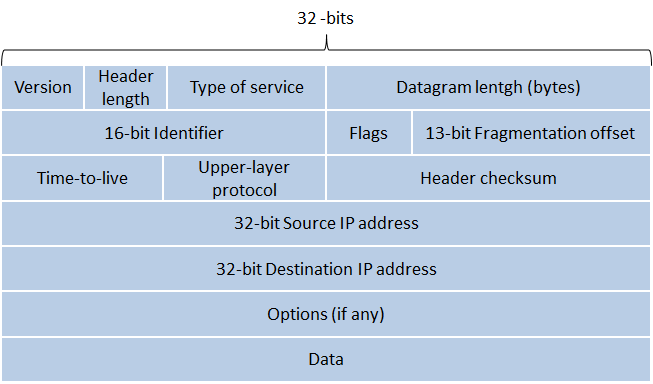
\includegraphics{4-network-layer/IPv4_datagram.png}
\begin{itemize}
	\item Versionsnummeret - 4 bit
	\item Headerlængde - 4 bit
	\item Servicetype (Type Of Service – TOS)
	\item Datagrammets længde
	\item Identifikation, flag og start på opdeling
	\item Time-to-live (TTL)
	\item Protokol i højere lag
	\item Headerens kontrolsum
	\item Afsender og modtageradresse
	\item Indstillinger
	\item Data
	\item Fragmentering af IP datagrammer(MTU Max Transfer Unit - 1500 ethernet, 576 WAN - identification flag - fragmentation offset fields - fragmentering  linklaget - leveres til transportlaget) 
\end{itemize}

\section{ICMP – Internet Control Message Protocol}
\begin{center}
  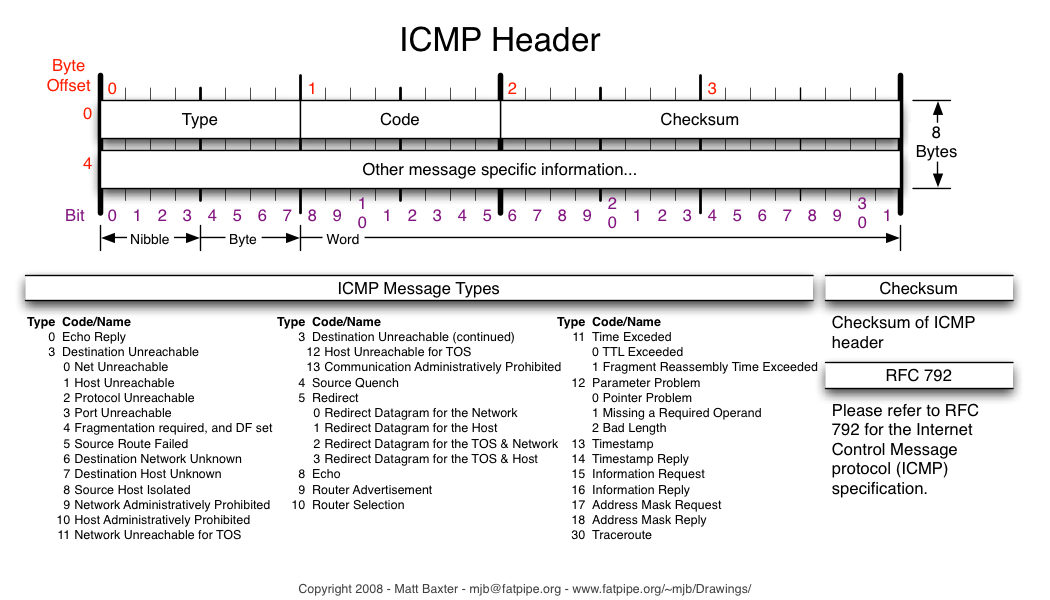
\includegraphics[scale=0.7]{4-network-layer/ICMP-Header.png}
\end{center}
\begin{itemize}
	\item værter, routere og gateways
	\item Fejlmeddelelser (Network unreachable f.eks. ftp, http og telnet session)
	\item Fragtes i IP datagrammer
	\item IP Datagram med ICMP videresendes ICMP
	\item Type
	\item Kode
	\item 8 bytes af IP datagrammet som foreårsagede fejlen
	\item eks. Ping
	\item eks. Traceroute
\end{itemize}
{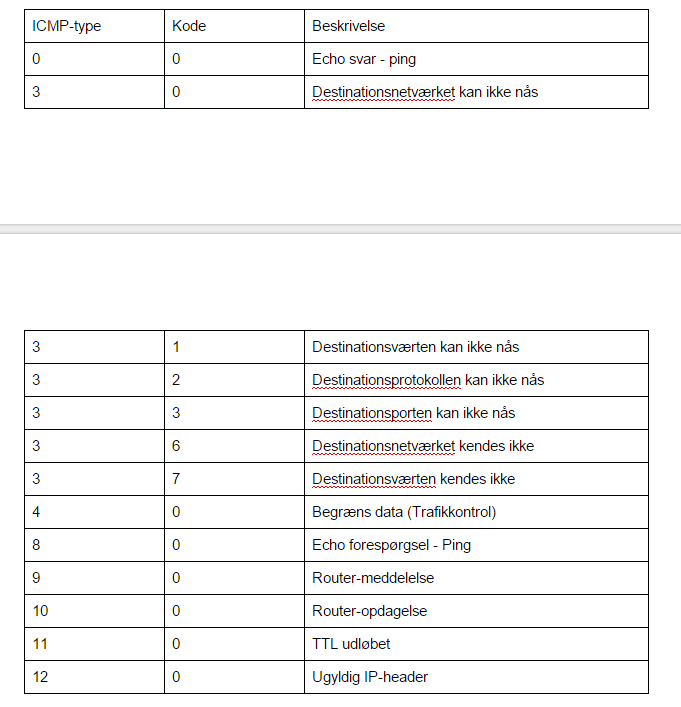
\includegraphics{4-network-layer/icmp-tabel.png}

\section{Network Address Translators - NAT}
NAT oversætter IP pakkerne således at de på ydersiden ser ud til at have en anden afsenderadresse (eller source/destination port) end maskinen, de oprindeligt kommer fra.
{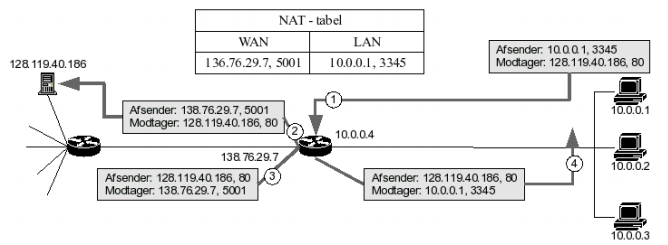
\includegraphics{4-network-layer/nat.png}
\begin{itemize}
	\item fremstå som 1 IP adresse
	\item se eksempel
	\item UPnP - Universal Plug and Play (simplificere hjemmenetværk - TCP/IP-protokollen)
\end{itemize}

\section{Routingprotokoller (Ikke en del af pensum)}
NAT oversætter IP pakkerne således at de på ydersiden ser ud til at have en anden afsenderadresse (eller source/destination port) end maskinen, de oprindeligt kommer fra.
\begin{itemize}
	\item RIP - Routing Information Protocol
	\item OSPF - Open Shortest Path First
	\item BGP - Border Gateway Protocol 
\end{itemize}
